\documentclass[12pt, a4paper]{article}

% --- ZÁKLADNÉ NASTAVENIA PODĽA ŠABLÓNY ---
\usepackage[utf8]{inputenc}
\usepackage[slovak]{babel}
\usepackage[T1]{fontenc}
\usepackage{mathptmx} % Písmo Times New Roman
\usepackage[left=3.5cm, right=2.5cm, top=2.5cm, bottom=2.5cm]{geometry} % Okraje podľa šablóny
\usepackage{setspace}
\onehalfspacing % Riadkovanie 1.5
\usepackage{graphicx}
\usepackage{titlesec}
\usepackage{indentfirst}
\usepackage{listings}
\usepackage{xcolor}
\usepackage{enumitem}
\usepackage{hyperref}
\usepackage{fancyhdr}
\usepackage{caption}

% Nastavenie odkazov a farieb
\hypersetup{
    colorlinks=true,
    linkcolor=black,
    filecolor=black,      
    urlcolor=black,
    citecolor=black
}

% Formátovanie nadpisov
\titleformat{\section}{\normalfont\fontsize{16}{19}\bfseries}{\thesection}{1em}{}
\titleformat{\subsection}{\normalfont\fontsize{14}{17}\bfseries}{\thesubsection}{1em}{}
\titleformat{\subsubsection}{\normalfont\fontsize{12}{15}\bfseries}{\thesubsubsection}{1em}{}

% Nastavenie päty pre číslovanie strán (vpravo dole)
\pagestyle{fancy}
\fancyhf{}
\renewcommand{\headrulewidth}{0pt}
\fancyfoot[R]{\thepage}

\begin{document}

% --- STRANA 1: OBAL ---
\begin{titlepage}
% horná hlavička školy
\begin{center}
\textbf{\large STREDNÁ PRIEMYSELNÁ ŠKOLA}\
\textbf{\large ELEKTROTECHNICKÁ}\
\textbf{\small ZOCHOVA 9, BRATISLAVA}
\end{center}

% veľká medzera do stredu strany
\vspace{3cm}
\begin{figure}[h]
    \centering
    \includegraphics[width=0.3\textwidth]{logo_2.png}
\end{figure}
\vspace{3cm}


% medzera k spodnej časti
\vfill

% spodná tabuľka s údajmi – zarovnanie ako v origináli
\noindent
\begin{tabular}{@{}ll@{\hspace{2cm}}ll}
Meno kandidáta: & Ján Dobák & Trieda: & IV.C \\
Vedúci práce: & Lenka Magndaléna Ráčková & Šk. rok: & 2025/2026
\end{tabular}

\vspace*{2.5cm}

\thispagestyle{empty}


% medzera k spodnej časti
\vfill



% --- STRANA 2: TITULNÝ LIST ---
\newpage
\thispagestyle{empty}
\begin{center}
    \large\textbf{STREDNÁ PRIEMYSELNÁ ŠKOLA ELEKTROTECHNICKÁ} \\
    \large\textbf{ZOCHOVA 9, BRATISLAVA}
    
    \vspace{6cm}
    {\Large\textbf{ProMAT - Projektový Manažment Systém}}
    \vspace{6cm}
    
    \begin{flushleft}
    \textbf{Meno kandidáta:} Ján Dobák \\
    \textbf{Vedúci práce:} Lenka Magdaléna Ráčková \\
    \textbf{Rozsah:} \pageref{LastPage} 
    \textbf{Odovzdané:} [Dátum] \\
    \textbf{Trieda:} [4.C] \\
    \vspace{1cm}
    \textbf{Podpis vedúceho práce:} \underline{\hspace{5cm}}
    \end{flushleft}
\end{center}

% --- STRANA 3: ORIGINÁL ZADANIA ---
\newpage
\thispagestyle{empty}
\begin{center}
    \vspace*{8cm}
    \textit{Tu bude vložený ORIGINÁL ZADANIA, ktorý si prevezmete na vrátnici.\\
    (Túto stranu v elektronickej verzii ponechajte ako placeholder alebo odstráňte pred tlačou)}
\end{center}

% --- STRANA 4: ČESTNÉ PREHLÁSENIE ---
\newpage
\thispagestyle{empty}
\vspace*{10cm}
\section*{Čestné prehlásenie}
Čestne prehlasujem, že problematiku týkajúcu sa náplne zadaného projektu v rámci praktickej časti odbornej zložky maturitnej skúšky formou obhajoby sme spracovali sami za pomoci uvedenej použitej literatúry. Inú, ako uvedenú literatúru sme nepoužili.

\vspace{2cm}
\noindent V Bratislave dňa: [Dátum] \hfill ...........................................\\
\hspace*{10cm} Ján Dobák

% --- STRANA 5: POĎAKOVANIE ---
\newpage
\thispagestyle{empty}
\vspace*{10cm}
\section*{Poďakovanie}
Chceli by sme sa poďakovať svojmu vedúcemu práce Lenke Magndaléne Ráčkovej za odborné vedenie, cenné rady a pripomienky, ktoré nám pomohli pri vypracovaní tohto projektu. Taktiež ďakujeme všetkým, ktorí nás podporovali počas štúdia.

% --- STRANA 6: OBSAH ---
\newpage
\thispagestyle{empty}
\tableofcontents

% --- STRANA 7, 8, 9: ZOZNAMY ---
\newpage
\thispagestyle{empty}
\listoffigures
\vspace{1cm}
\listoftables

\newpage
\thispagestyle{empty}
\section*{ZOZNAM SKRATIEK}
\begin{tabular}{ll}
\textbf{Skratka} & \textbf{Popis} \\
AI & Umelá inteligencia (Artificial Intelligence) \\
SQL & Structured Query Language \\
RAG & Retrieval-Augmented Generation \\
LLM & Large Language Model \\
FTS & Full-Text Search \\
UI & User Interface (Používateľské rozhranie) \\
REST & Representational State Transfer \\
HTTP & Hypertext Transfer Protocol \\
WSGI & Web Server Gateway Interface \\
ACID & Atomicity, Consistency, Isolation, Durability \\
\end{tabular}

% --- HLAVNÝ TEXT (ZAČÍNA STRANA 1) ---
\newpage
\setcounter{page}{1}

\section{Úvod}

\subsection{Motivácia a cieľ práce}
V súčasnej dobe, keď práca v tímoch a manažment projektov predstavuje kľúčový aspekt každej modernej organizácie, vzniká potreba efektívnych nástrojov na koordináciu aktivít, sledovanie úloh a správu dokumentácie. Projekt \textbf{ProMAT (Project Management Tool)} bol vytvorený ako odpoveď na tieto potreby.

Hlavným cieľom tohto projektu je vyvinúť komplexný interný systém pre projektový manažment, ktorý kombinuje tradičné funkcie správy projektov s modernými technológiami umelej inteligencie. Systém je určený pre malé a stredné tímy, ktoré potrebujú centralizované riešenie pre:

\begin{itemize}
    \item Správu projektov a ich životného cyklu od inicializácie po ukončenie.
    \item Organizáciu a sledovanie úloh (task management) pomocou vizuálnych nástrojov.
    \item Správu dokumentov s možnosťou inteligentného vyhľadávania a analýzy obsahu.
    \item Kolaboráciu členov tímu v reálnom čase s podporou prideľovania rolí.
\end{itemize}

\subsection{Špecifikácia problému}
Existujúce riešenia na trhu (ako Jira, Trello, Asana) sú často príliš komplexné, finančne nákladné alebo neposkytujú dostatočnú flexibilitu pre menšie organizácie, ktoré preferujú on-premise riešenia. Navyše, väčšina z nich nepodporuje natívne inteligentné spracovanie dokumentov pomocou AI bez nutnosti odosielať dáta tretím stranám.

Tento projekt rieši tieto problémy poskytnutím:
\begin{enumerate}
    \item \textbf{Jednoduchého a intuitívneho rozhrania} - Moderný dizajn zameraný na používateľskú prívetivosť (User Experience).
    \item \textbf{Lokálneho behu} - Aplikácia beží úplne lokálne, čo zvyšuje bezpečnosť citlivých firemných dát.
    \item \textbf{AI integrácie} - Integrovaný chatbot pre inteligentné dotazy nad dokumentmi využíva lokálne LLM modely.
    \item \textbf{Multi-tenancy} - Podpora viacerých nezávislých organizácií v rámci jednej inštancie aplikácie.
\end{enumerate}

\newpage
\section{Teoretický základ}

Táto kapitola sa venuje teoretickému rozboru technológií, metodík a princípov, ktoré boli využité pri návrhu a implementácii systému ProMAT. Dôraz je kladený na vysvetlenie fungovania webových rámcov, databázových systémov a moderných prístupov v oblasti umelej inteligencie.

\subsection{Metodiky vývoja softvéru a projektový manažment}
Pri vývoji softvéru je kľúčové zvoliť správnu metodiku, ktorá definuje procesy, roly a postupy práce. Systém ProMAT je navrhnutý tak, aby podporoval moderné agilné metodiky.

\subsubsection{Agilný prístup vs. Tradičný model}
Tradičný vodopádový model (Waterfall) je charakteristický lineárnym postupom, kde jedna fáza začína až po skončení predchádzajúcej. Tento prístup je často nepružný voči zmenám požiadaviek. Naopak, agilný prístup (Agile) je iteračný a inkrementálny. Umožňuje rýchlu reakciu na zmeny a kladie dôraz na komunikáciu v tíme a funkčný softvér. V našom projekte sme aplikovali agilné princípy, čo sa odrazilo aj vo funkcionalite samotnej aplikácie (napr. možnosť rýchlej zmeny priorít úloh).

\subsubsection{Metodika Kanban}
Kanban je vizuálny systém na riadenie práce, ktorý sa snaží o maximalizáciu efektivity a plynulosti toku práce (flow). Základom je Kanban tabuľa (Board), ktorá vizualizuje pracovné položky v rôznych stavoch (stĺpcoch). Typické stĺpce sú \textit{To Do}, \textit{In Progress} a \textit{Done}.

Kľúčové princípy Kanbanu, ktoré sme implementovali v systéme ProMAT:
\begin{itemize}
    \item \textbf{Vizualizácia práce:} Každá úloha je reprezentovaná kartou na tabuli.
    \item \textbf{Obmedzenie rozpracovanej práce (WIP):} Prevencia preťaženia členov tímu.
    \item \textbf{Riadenie toku:} Sledovanie, ako rýchlo sa úlohy presúvajú medzi stavmi.
\end{itemize}

\subsection{Webové technológie a architektúra}
Aplikácia ProMAT je postavená na architektúre klient-server, ktorá je štandardom pre moderné webové aplikácie.

\subsubsection{Protokol HTTP a REST princípy}
Komunikácia medzi klientom (prehliadačom) a serverom prebieha prostredníctvom protokolu HTTP (Hypertext Transfer Protocol). Tento bezstavový protokol definuje metódy ako GET (získanie dát), POST (odoslanie dát), PUT (aktualizácia) a DELETE (vymazanie).
Naša aplikácia dodržiava princípy REST (Representational State Transfer), čo znamená, že zdroje (napr. projekty, úlohy) sú identifikovateľné pomocou URL adries a operácie nad nimi využívajú štandardné HTTP metódy. To zabezpečuje prehľadnosť a ľahkú rozšíriteľnosť systému.

\subsection{Aplikačný rámec Flask}
Flask je mikroframework pre jazyk Python, ktorý poskytuje základné nástroje na vytváranie webových aplikácií bez vynútenia striktnej štruktúry projektu. Bol zvolený pre svoju jednoduchosť, flexibilitu a rozsiahlu komunitu.

\subsubsection{Architektúra a filozofia Flasku}
Na rozdiel od "full-stack" frameworkov ako Django, Flask neobsahuje v jadre nástroje pre prácu s databázou či validáciu formulárov. Namiesto toho je navrhnutý tak, aby bol rozšíriteľný pomocou externých knižníc. Jadro Flasku závisí na dvoch hlavných komponentoch:
\begin{itemize}
    \item \textbf{Werkzeug:} Knižnica pre WSGI (Web Server Gateway Interface), ktorá zabezpečuje komunikáciu medzi webovým serverom a Python aplikáciou. Rieši smerovanie (routing), ladenie a prácu s požiadavkami.
    \item \textbf{Jinja2:} Moderný a bezpečný šablónovací systém pre Python.
\end{itemize}

\subsubsection{Šablónovací systém Jinja2}
Jinja2 umožňuje oddeliť logiku aplikácie od jej prezentačnej vrstvy (HTML). Podporuje dedičnosť šablón, čo výrazne redukuje duplicitu kódu. V projekte ProMAT využívame základnú šablónu \texttt{base.html}, ktorá obsahuje spoločné prvky (hlavička, menu, pätička), a do nej vkladáme obsah konkrétnych stránok. Jinja2 tiež zabezpečuje automatické "escapovanie" výstupov, čím chráni aplikáciu pred útokmi typu XSS (Cross-Site Scripting).

\subsubsection{Spracovanie požiadaviek a Blueprints}
Flask spracováva HTTP požiadavky mapovaním URL adries na Python funkcie (tzv. views). Pre lepšiu organizáciu kódu vo väčších aplikáciách Flask ponúka mechanizmus \textit{Blueprints}. Blueprints umožňujú rozdeliť aplikáciu na menšie, logické celky (napr. modul pre autentifikáciu, modul pre projekty, modul pre API), ktoré je možné vyvíjať a spravovať samostatne.

\subsection{Databázové systémy a SQLite}
Dáta sú neoddeliteľnou súčasťou každej informačnej systémy. Pre potreby projektu ProMAT sme zvolili relačnú databázu SQLite.

\subsubsection{Relačný model a SQL}
Relačný model organizuje dáta do tabuliek (relácií), ktoré pozostávajú z riadkov (záznamov) a stĺpcov (atribútov). Vzťahy medzi tabuľkami sú realizované pomocou primárnych a cudzích kľúčov. Na manipuláciu s dátami sa využíva jazyk SQL (Structured Query Language). Pri návrhu databázy sme dbali na normalizáciu, aby sme predišli redundancii dát a anomáliám pri aktualizácii.

\subsubsection{Vlastnosti a výhody SQLite}
SQLite je serverless, self-contained databázový engine. Na rozdiel od systémov ako PostgreSQL alebo MySQL nevyžaduje bežiaci serverový proces. Celá databáza je uložená v jedinom súbore na disku.
\begin{itemize}
    \item \textbf{Zero-configuration:} Nie je potrebná inštalácia ani konfigurácia servera.
    \item \textbf{ACID kompatibilita:} SQLite garantuje atomicitu, konzistenciu, izoláciu a trvácnosť transakcií, čo je kľúčové pre integritu dát aj pri výpadku prúdu či páde aplikácie.
    \item \textbf{Portabilita:} Súbor databázy je prenositeľný medzi rôznymi operačnými systémami.
\end{itemize}

\subsubsection{Full-Text Search (FTS)}
Pre efektívne vyhľadávanie v obsahu dokumentov sme využili rozšírenie SQLite FTS5. Toto rozšírenie vytvára virtuálne tabuľky, ktoré umožňujú rýchle fulltextové vyhľadávanie v textových dátach, čo je podstatne efektívnejšie ako použitie štandardného operátora \texttt{LIKE}.

\subsection{Umelá inteligencia a spracovanie prirodzeného jazyka (NLP)}
Jednou z hlavných inovácií v systéme ProMAT je integrácia umelej inteligencie pre prácu s dokumentmi.

\subsubsection{Veľké jazykové modely (LLM)}
LLM (Large Language Models) sú neurónové siete trénované na obrovskom množstve textových dát. Sú schopné porozumieť kontextu, generovať text, prekladať a odpovedať na otázky. Moderné LLM sú založené na architektúre \textbf{Transformer}, ktorá využíva mechanizmus pozornosti (self-attention) na spracovanie vzťahov medzi slovami v texte, bez ohľadu na ich vzdialenosť vo vete.

\subsubsection{Vektorové vnorenia (Embeddings)}
Prepojenie textu s matematickými operáciami umožňujú tzv. embeddings. Ide o prevod textu (slova, vety alebo odseku) na číselný vektor s pevnou dimenziou (napr. 768 čísel). V tomto vektorovom priestore platí, že sémanticky podobné texty majú vektory, ktoré sú si blízke (majú malú uhlovú vzdialenosť). Tento princíp využívame pri vyhľadávaní relevantných častí dokumentov na základe používateľskej otázky.

\subsubsection{Retrieval-Augmented Generation (RAG)}
RAG je technika, ktorá kombinuje schopnosti generatívnych modelov s externou znalostnou bázou. Rieši problém "halucinácií" LLM, kedy model vymýšľa fakty, a problém neaktuálnosti trénovacích dát.
Proces RAG v našej aplikácii:
\begin{enumerate}
    \item \textbf{Ingestion:} Dokument sa rozdelí na menšie časti (chunks) a prevedie na vektory.
    \item \textbf{Retrieval (Vyhľadávanie):} Otázka používateľa sa prevedie na vektor a v databáze sa nájdu najpodobnejšie časti dokumentov (kontext).
    \item \textbf{Generation (Generovanie):} Nájdený kontext sa spolu s otázkou vloží do promptu pre LLM, ktorý vygeneruje odpoveď založenú výlučne na poskytnutých informáciách.
\end{enumerate}

\subsubsection{Lokálny beh modelov (Ollama)}
Z dôvodu ochrany súkromia a nezávislosti od internetu využívame platformu Ollama. Tá umožňuje spúšťať kvantizované verzie modelov (napr. Llama 2, Mistral) priamo na hardvéri používateľa. Kvantizácia znižuje pamäťovú náročnosť modelov znížením presnosti váh (napr. z 16-bit na 4-bit) s minimálnym dopadom na kvalitu výstupu, čo umožňuje beh pokročilej AI aj na bežných notebookoch.

\newpage
\section{Analýza a návrh systému}

\subsection{Funkčné požiadavky}
Na základe analýzy potrieb cieľovej skupiny sme definovali nasledujúce funkčné požiadavky:
\begin{itemize}
    \item \textbf{Správa používateľov:} Systém umožňuje registráciu, prihlásenie a správu používateľského účtu. Súčasťou riešenia je prideľovanie rolí na úrovni celej aplikácie aj na úrovni jednotlivých projektov.
    \item \textbf{Správa projektov:} Používateľ môže vytvárať, upravovať, archivovať a odstraňovať projekty. Každý projekt obsahuje vlastný kontext, členov, úlohy, dokumenty a plánovacie artefakty.
    \item \textbf{Správa tímu:} Pre každý projekt vieme evidovať členov a ich oprávnenia (viewer, member, manager, admin), čím je možné jemnejšie riadiť editácie a schvaľovanie zmien.
    \item \textbf{Správa úloh:} Úlohy obsahujú názov, popis, prioritu, stav, termín, zodpovednú osobu, značky, komentáre, prílohy, checklist a závislosti. V rámci tímovej práce podporujeme tabuľkový aj kanban pohľad.
    \item \textbf{Plánovanie sprintov a backlogu:} Úlohy môžeme zoskupovať do sprintov, presúvať medzi backlogom a aktívnym sprintom a sledovať ich priebeh počas iterácie.
    \item \textbf{Notifikácie a sledovanie aktivít:} Používateľ dostáva notifikácie o zmenách úloh (priradenie, zmienka, termín), pričom systém zaznamenáva históriu dôležitých operácií.
    \item \textbf{Správa dokumentov:} Aplikácia podporuje upload súborov PDF a DOCX, extrakciu textu, verzovanie dokumentov, tagovanie a následné vyhľadávanie relevantných častí obsahu.
    \item \textbf{AI podpora nad dokumentmi:} Používateľ môže klásť otázky nad obsahom dokumentov, žiadať stručné zhrnutie a získavať odpovede s uvedením kontextových úryvkov.
    \item \textbf{Integrácie a export:} Súčasťou riešenia je import a export údajov (napr. CSV) a webhook rozhranie pre napojenie na externé procesy.
\end{itemize}

\subsection{Používateľské roly a scenáre používania}
Pri návrhu sme vychádzali z toho, že v jednom tíme pracujú používatelia s rôznou zodpovednosťou. Preto sme navrhli dvojúrovňový model oprávnení: globálna rola používateľa a projektová rola člena.

\subsubsection{Globálne roly}
Globálne roly reprezentujú základné oprávnenia v celej aplikácii. Typicky ide o administrátora, vlastníka alebo člena tímu s obmedzeným rozsahom práv. Tento model nám umožňuje jednoducho oddeliť manažérske úkony (správa používateľov, systémové nastavenia) od bežnej dennej práce.

\subsubsection{Projektové roly}
Na úrovni projektu evidujeme roly \textit{viewer}, \textit{member}, \textit{manager} a \textit{admin}. Tento mechanizmus je dôležitý najmä v situácii, keď má jeden používateľ v rôznych projektoch odlišné postavenie. Napríklad v jednom projekte môže iba čítať stav, v inom môže riadiť backlog, sprinty a členov tímu.

\subsubsection{Kľúčové používateľské scenáre}
Počas analýzy sme identifikovali najčastejšie scenáre práce:
\begin{enumerate}
    \item \textbf{Založenie projektu a tímu:} Vedúci tímu vytvorí projekt, priradí členov a nastaví ich projektové roly.
    \item \textbf{Príprava backlogu:} Členovia tímu vytvoria sadu úloh, doplnia priority, termíny a odhadnú poradie realizácie.
    \item \textbf{Realizácia práce v Kanban/Sprint režime:} Úlohy sa priebežne presúvajú medzi stavmi, dopĺňajú sa komentáre, checklisty a prílohy.
    \item \textbf{Práca s dokumentáciou:} K projektu sa nahrávajú dokumenty, ktoré systém spracuje a pripraví pre inteligentné dotazovanie.
    \item \textbf{AI konzultácia nad obsahom:} Používateľ otvorí chat, položí otázku a dostane odpoveď opretú o textové úryvky z dokumentov.
    \item \textbf{Uzavretie iterácie:} Po ukončení sprintu tím vyhodnotí stav úloh, presunie nedokončené položky späť do backlogu a pripraví ďalší cyklus.
\end{enumerate}

\subsection{Návrh doménového modelu}
Návrh dátového modelu sme postavili na relačnom základe s jasne definovanými väzbami medzi hlavnými entitami. Cieľom bolo dosiahnuť konzistentné ukladanie údajov pri zachovaní flexibility pre ďalšie rozširovanie.

\subsubsection{Hlavné entity systému}
\begin{itemize}
    \item \textbf{User:} reprezentuje používateľa systému, jeho identitu, rolu a väzby na projekty, úlohy, notifikácie a AI chat.
    \item \textbf{Project:} predstavuje kontajner pre tímovú prácu. Združuje úlohy, dokumenty, sprinty, členstvá a nastavenia tabule.
    \item \textbf{Task:} jadro operatívneho riadenia práce. Okrem základných atribútov obsahuje väzby na checklist položky, značky, komentáre, prílohy, aktivitu a sprint.
    \item \textbf{Document:} uchováva metadáta súboru, extrahovaný text, tagy a väzbu na projekt, vďaka čomu môžeme nad dokumentom vykonávať AI operácie.
    \item \textbf{ChatSession a ChatMessage:} modelujú konverzáciu používateľa s AI vrstvou, vrátane historizácie otázok a odpovedí.
    \item \textbf{Sprint a planning entity:} entita sprintu, uložené filtre, členstvá, notifikácie, watcher väzby, automatizačné pravidlá a API tokeny.
\end{itemize}

\subsubsection{Vzťahy medzi entitami}
Medzi entitami sme definovali väzby typu 1:N aj N:M. Používateľ môže byť členom viacerých projektov, pričom projekt má viac členov. Podobne projekt obsahuje viac úloh a viac dokumentov. Úloha môže mať viaceré komentáre, značky či prílohy. Tento model umožňuje prirodzene pokryť reálnu tímovú spoluprácu bez umelej duplicity záznamov.

Pri návrhu sme dbali na to, aby väzby odrážali aj životný cyklus objektov. Ak je napríklad odstránený projekt, súvisiace záznamy (úlohy, dokumenty, členstvá) sa spracujú konzistentne podľa nastavených pravidiel väzieb. Tým predchádzame stavu, keď by v databáze zostávali osirelé dáta bez vlastníka.

\subsection{Návrh procesných tokov}
Procesné toky sme navrhli ako postupnosť krokov, ktoré používateľ vykonáva v prirodzenom poradí počas práce na projekte. Cieľom bolo minimalizovať počet prepnutí medzi obrazovkami a zároveň zachovať prehľadnosť.

\subsubsection{Tok správy úloh}
Základný tok začína vytvorením úlohy. Používateľ doplní názov, projekt, prioritu, stav, termín a zodpovednú osobu. Následne môže úlohu dopĺňať o komentáre, checklist a prílohy. V kanban zobrazení sa úloha presúva medzi stĺpcami, čo predstavuje zmenu stavu v doménovom modeli. Každá významná zmena sa zapíše do aktivity, aby bolo možné spätne dohľadať priebeh riešenia.

\subsubsection{Tok plánovania sprintu}
Pri plánovaní tím najskôr pripraví backlog. Vybrané úlohy sa priradia do sprintu, ktorý má názov, cieľ a časové ohraničenie. Počas trvania sprintu sledujeme stav úloh a po uzavretí sprintu vyhodnotíme dokončené a nedokončené položky. Nedokončené úlohy sa vracajú do backlogu alebo sa presúvajú do ďalšieho sprintu.

\subsubsection{Tok práce s dokumentom a AI chatom}
Používateľ nahrá dokument, systém ho uloží, extrahuje text a sprístupní ho pre vyhľadávanie. Pri otázke v AI chate sa najskôr nájdu relevantné úseky textu, následne sa vytvorí kontext pre model a až potom sa generuje odpoveď. Týmto spôsobom držíme odpoveď v hraniciach dostupných podkladov a zároveň skracujeme čas, ktorý by používateľ inak strávil manuálnym hľadaním informácií.

\subsection{Návrh AI vrstvy nad dokumentmi}
AI vrstvu sme navrhli ako samostatnú službu, ktorú možno ďalej rozširovať bez zásahu do jadra doménových entít. Tento prístup podporuje modulárnosť riešenia a jasné oddelenie zodpovedností.

\subsubsection{Požadované AI operácie}
Z pohľadu funkcií sme definovali tri hlavné operácie:
\begin{itemize}
    \item \textbf{Chat nad dokumentmi:} odpovedanie na používateľské otázky na základe nájdených pasáží.
    \item \textbf{Sumarizácia:} vytvorenie stručného prehľadu obsahu dokumentu.
    \item \textbf{Sémantické hľadanie pojmov:} identifikácia relevantných častí dokumentov pre konkrétny výraz alebo tému.
\end{itemize}

\subsubsection{Návrhové princípy AI integrácie}
Pri návrhu sme dodržali tieto zásady:
\begin{enumerate}
    \item AI vrstva je volaná cez jasne definované servisné rozhranie.
    \item Chat správy sa ukladajú do databázy ako samostatné entity pre spätné dohľadanie kontextu.
    \item Odpoveď sa tvorí až po výbere relevantných pasáží z dokumentov, nie izolovane bez podkladov.
    \item AI funkcie sú navrhnuté tak, aby bolo možné neskôr vymeniť model alebo spôsob retrieval bez zásadného zásahu do UI vrstvy.
\end{enumerate}


\newpage
\section{Implementácia}

\subsection{Štruktúra projektu}
Zdrojový kód je organizovaný do modulárnej štruktúry, čo uľahčuje údržbu a orientáciu v projekte.
\begin{verbatim}
ProMAT/
├── config.py
├── run.py
├── seed.py
├── requirements.txt
├── app/
│   ├── __init__.py
│   ├── extensions.py
│   ├── blueprints/
│   ├── models/
│   ├── services/
│   ├── templates/
│   └── static/
├── documentation/
└── uploads/
\end{verbatim}

Aktuálna štruktúra reflektuje architektúru založenú na \textit{application factory} prístupe vo Flasku. Vstupný bod \texttt{run.py} inicializuje aplikáciu, pričom konfigurácia prostredia je centralizovaná v súbore \texttt{config.py}. Týmto spôsobom vieme jednoducho oddeľovať prostredia a udržať konzistentné štartovanie aplikácie.

\subsection{Aplikačné jadro a Blueprints}
Súbor \texttt{app/\_\_init\_\_.py} implementuje továrenskú funkciu na vytvorenie Flask aplikácie. V tejto fáze inicializujeme rozšírenia (databáza, prihlásenie, ochrana formulárov) a registrujeme jednotlivé blueprinty.

Rozdelenie na blueprinty predstavuje kľúčovú organizačnú techniku:
\begin{itemize}
    \item \texttt{auth.py} pre autentifikáciu používateľov,
    \item \texttt{dashboard.py} pre hlavný prehľad,
    \item \texttt{projects.py}, \texttt{tasks.py}, \texttt{documents.py} pre doménové moduly,
    \item \texttt{ai\_chat.py} pre komunikáciu s AI vrstvou,
    \item \texttt{team.py} pre správu členov a rolí.
\end{itemize}

Výhodou tohto prístupu je oddelenie URL routingu, validačnej logiky a renderovania šablón podľa domén. Pri ďalšom rozširovaní tak nevzniká monolitický súbor s ťažko udržiavateľným routingom.

\subsection{Implementácia autentifikácie}
Autentifikáciu sme postavili na mechanizmoch Flask-Login a Werkzeug. Heslá používateľov neukladáme v otvorenom tvare, ale vo forme hash hodnôt. Prístup k chráneným častiam je podmienený aktívnou reláciou.

Ochrana rout je realizovaná dekorátorom \texttt{login\_required}. Pri neautorizovanom prístupe používateľa presmerujeme na prihlasovaciu obrazovku. Tento mechanizmus vytvára jednotné pravidlo pre všetky moduly aplikácie.

\begin{lstlisting}[language=Python, frame=single, basicstyle=\footnotesize]
# Príklad implementácie dekorátora pre ochranu ciest
def login_required(f):
    @wraps(f)
    def decorated_function(*args, **kwargs):
        if 'user_id' not in session:
            flash('Pre prístup sa musíte prihlásiť.', 'warning')
            return redirect(url_for('login'))
        return f(*args, **kwargs)
    return decorated_function
\end{lstlisting}

Nad rámec samotného prihlásenia sme implementovali aj kontrolu rolí pri vybraných operáciách. Pri práci s tímom, nastaveniami projektu alebo úpravou citlivých údajov systém overuje, či má používateľ dostatočné oprávnenie v danom projekte.

\subsection{Implementácia dátovej vrstvy}
Dátová vrstva je postavená na SQLAlchemy ORM. Modely sú rozdelené do viacerých súborov podľa domény, čo zvyšuje čitateľnosť a uľahčuje správu väzieb.

\subsubsection{Modely jadra}
Do jadra patria modely \texttt{User}, \texttt{Project}, \texttt{Task}, \texttt{Document}, \texttt{Comment} a modely AI konverzácie. Každý model obsahuje nielen základné atribúty, ale aj explicitne definované vzťahy, ktoré využívame pri načítavaní údajov pre šablóny a API odpovede.

\subsubsection{Modely plánovania a spolupráce}
V samostatnom module plánovania evidujeme sprinty, členstvá projektu, notifikácie, watcher väzby, uložené filtre a pravidlá automatizácie. Tieto entity rozširujú základný task manažment na úroveň komplexnej tímovej koordinácie, pričom stále ostávame pri jednom konzistentnom databázovom modeli.

\subsection{Implementácia modulu úloh}
Modul úloh patrí medzi najrozsiahlejšie časti aplikácie. V blueprinte \texttt{tasks.py} sme spojili CRUD operácie, kanban workflow, sprint plánovanie, reporty, notifikácie a integrácie.

\subsubsection{Tabuľkový a kanban pohľad}
V tabuľkovom pohľade používateľ filtruje úlohy podľa projektu, stavu, zodpovednej osoby, značiek alebo rýchlych predvolieb (napr. moje úlohy, po termíne). Kanban pohľad pracuje so stĺpcami podľa stavu a podporuje drag-and-drop presuny.

Na obrázku nižšie je pripravené miesto pre finálny screenshot kanban tabule s rozdelením úloh podľa stavov.

\begin{figure}[h!]
    \centering
    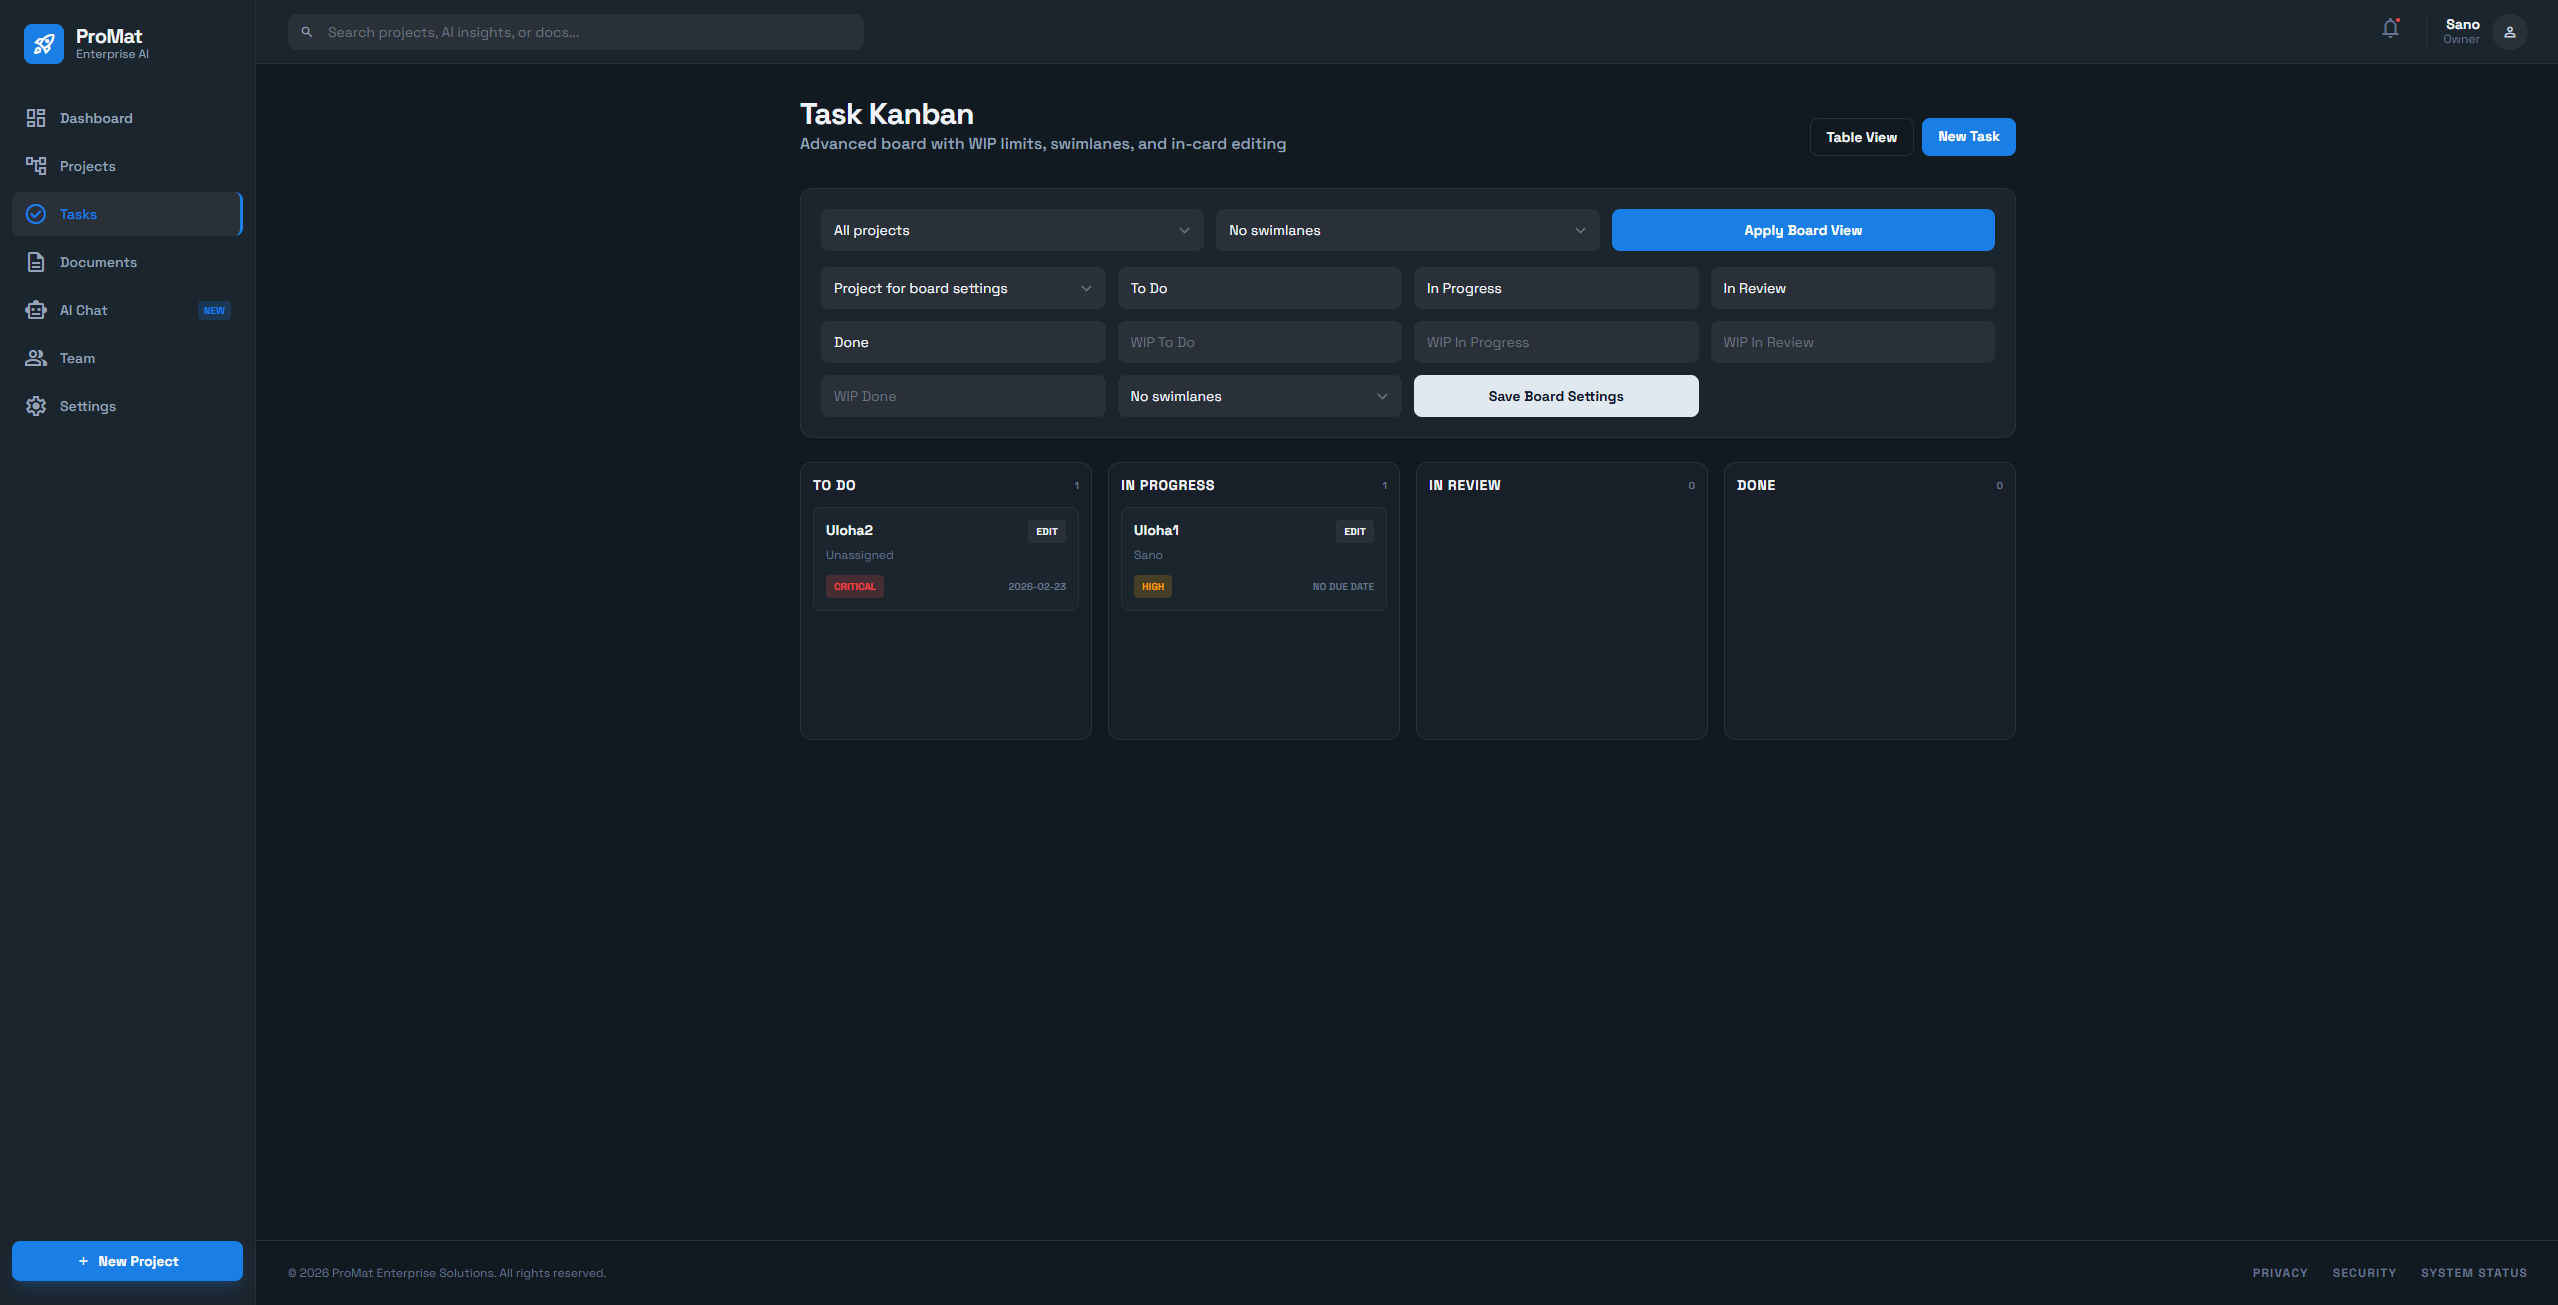
\includegraphics[width=0.95\textwidth]{kanban.png} 
    \caption{Kanban tabuľa modulu úloh}
    \label{fig:kanban}
\end{figure}

Špecifickou vlastnosťou je konfigurovateľnosť tabule: pre každý projekt môžeme upraviť názvy stĺpcov, WIP limity a režim swimlane. Vďaka tomu sa pracovný proces dokáže prispôsobiť konkrétnemu tímu bez potreby meniť kód aplikácie.

\subsubsection{Doplnkové funkcie úloh}
Každá úloha môže obsahovať:
\begin{itemize}
    \item checklist položky na jemnejšie rozdelenie práce,
    \item komentáre s priebežnou diskusiou,
    \item prílohy a odkazy,
    \item závislosti medzi úlohami,
    \item históriu aktivít pre spätnú rekonštrukciu priebehu.
\end{itemize}

Tento rozsah funkcií výrazne znižuje potrebu používať externé nástroje na komunikáciu a evidenciu detailov, pretože projektový kontext zostáva centralizovaný na jednom mieste.

\subsubsection{Sprinty, reporty a notifikácie}
V rámci plánovacej vrstvy sme implementovali správu sprintov (vytvorenie, aktivácia, uzavretie), reporty priebehu a centrum notifikácií. Reporty sumarizujú aktuálny stav práce a uľahčujú rozhodovanie vedúceho projektu pri plánovaní ďalšej iterácie.

Notifikácie sú naviazané na udalosti v systéme, ako je priradenie úlohy, zmena stavu alebo zmienka v komentári. Používateľ tak nemusí manuálne kontrolovať všetky projekty, ale dostáva prehľad o udalostiach, ktoré sa ho týkajú.

\subsection{Implementácia správy dokumentov}
Dokumentový modul sme navrhli tak, aby bol použiteľný aj bez AI funkcií, no zároveň pripravený na ich okamžité využitie.

\subsubsection{Upload a extrakcia textu}
Po nahratí súboru systém vykoná kontrolu typu prípony, uloží súbor na disk a podľa formátu zavolá vhodnú extrakčnú funkciu. Pri PDF využívame \texttt{PyPDF2}, pri DOCX knižnicu \texttt{python-docx}. Extrahovaný text ukladáme priamo k záznamu dokumentu, čo zjednodušuje následné vyhľadávanie a spracovanie.

Súčasťou procesu je aj verzovanie dokumentov v rámci projektu, vďaka čomu vieme pracovať s postupne aktualizovanými podkladmi bez straty histórie.

\subsubsection{Zobrazenie a filtrovanie dokumentov}
Používateľ má k dispozícii zoznam dokumentov s filtráciou podľa projektu, typu súboru, tagov a textového hľadania podľa názvu. Detail dokumentu obsahuje metadáta, extrahovaný text a akcie na stiahnutie alebo otvorenie AI chatu.

Takto navrhnutý tok umožňuje prejsť od nahratia dokumentu po položenie otázky v minimálnom počte krokov.

\subsection{Služba RAG (Retrieval-Augmented Generation)}
Inteligentná vrstva je implementovaná servisným spôsobom. V aktuálnej verzii obsahuje základné AI operácie (chat, sumarizácia, sémantické vyhľadávanie) s jasne definovaným rozhraním, na ktoré je naviazaný blueprint \texttt{ai\_chat.py}.

Architektúra AI časti je postavená na princípe „najprv kontext, potom odpoveď“. Pred samotným generovaním preto pripravíme vstupné pasáže z dokumentov a tieto vložíme do promptu. Tým dosahujeme, že odpoveď sa opiera o interné podklady projektu.

Nasledujúca ukážka reprezentuje princíp skladania promptu a volania modelu:

\begin{lstlisting}[language=Python, frame=single, basicstyle=\footnotesize]
def generate_chat_response(query, context_chunks):
    """
    Generuje odpoveď pomocou LLM na základe nájdeného kontextu.
    """
    context = '\n\n'.join(context_chunks)
    # Prompt engineering - inštrukcie pre model
    prompt = f"""
    Použi nasledujúci kontext na zodpovedanie otázky.
    Ak odpoveď nie je v kontexte, povedz, že nevieš.
    
    Kontext: {context}
    Otázka: {query}
    """
    
    response = requests.post(
        'http://localhost:11434/api/generate',
        json={'model': 'llama3', 'prompt': prompt, 'stream': False}
    )
    return response.json()['response']
\end{lstlisting}

\subsubsection{Praktický workflow RAG v aplikácii}
Reálny workflow môžeme zhrnúť do nasledujúcich krokov:
\begin{enumerate}
    \item Používateľ vyberie dokument alebo projektový kontext, nad ktorým chce pracovať.
    \item Systém vyhľadá najrelevantnejšie textové pasáže podľa otázky.
    \item Tieto pasáže sa spoja do kontextového bloku a odošlú modelu spolu s otázkou.
    \item Výsledná odpoveď sa uloží do histórie konverzácie a zobrazí sa používateľovi v chat rozhraní.
\end{enumerate}

Na obrázku nižšie je priestor pre ukážku AI chatu nad dokumentmi, kde je viditeľný dotaz používateľa a odpoveď modelu s kontextom.

\begin{figure}[h!]
    \centering
    
\includegraphics[width=0.95\textwidth]{ai_chat.png}
    \caption{AI chat nad projektovou dokumentáciou}
    \label{fig:ai-chat}
\end{figure}

Výhodou tohto prístupu je, že používateľ nemusí manuálne prechádzať rozsiahle dokumenty. Namiesto toho získava stručnú odpoveď s oporou v nájdenom texte, pričom konverzácia zostáva naviazaná na konkrétny projekt.

\subsection{Integrácie a automatizácia}
V implementácii sme počítali aj s prepojením na externé nástroje. Modul úloh preto obsahuje API tokeny a webhook endpointy, cez ktoré je možné odosielať alebo prijímať udalosti (napr. zmena stavu úlohy, vytvorenie novej položky).

Okrem toho sme pridali pravidlá automatizácie vo forme \textit{if-then} scenárov. Pri splnení definovanej podmienky sa vykoná akcia, napríklad priradenie používateľa, zmena stavu alebo doplnenie značky. Tento mechanizmus redukuje rutinné operácie a zvyšuje konzistenciu procesov v tíme.

\subsection{Používateľské rozhranie (Frontend)}
Prezentačná vrstva je postavená na Jinja2 šablónach, Tailwind CSS a čistom JavaScripte. Dizajn je konzistentne orientovaný na tmavý režim, pričom jednotlivé stránky zdieľajú spoločný layout cez \texttt{base.html}.

\subsubsection{Komponentový prístup v šablónach}
Rozhranie sme rozdelili na opakovane použiteľné komponenty (sidebar, header, footer, karty štatistík, riadky tabuliek, modálne okná). Tento prístup znižuje duplicitu a uľahčuje jednotnú úpravu dizajnu naprieč modulmi.

Pre finálnu verziu dokumentácie je pripravené aj miesto pre screenshot hlavného dashboardu, ktorý bude vizuálne demonštrovať jednotný dizajnový jazyk aplikácie.

\begin{figure}[h!]
    \centering
    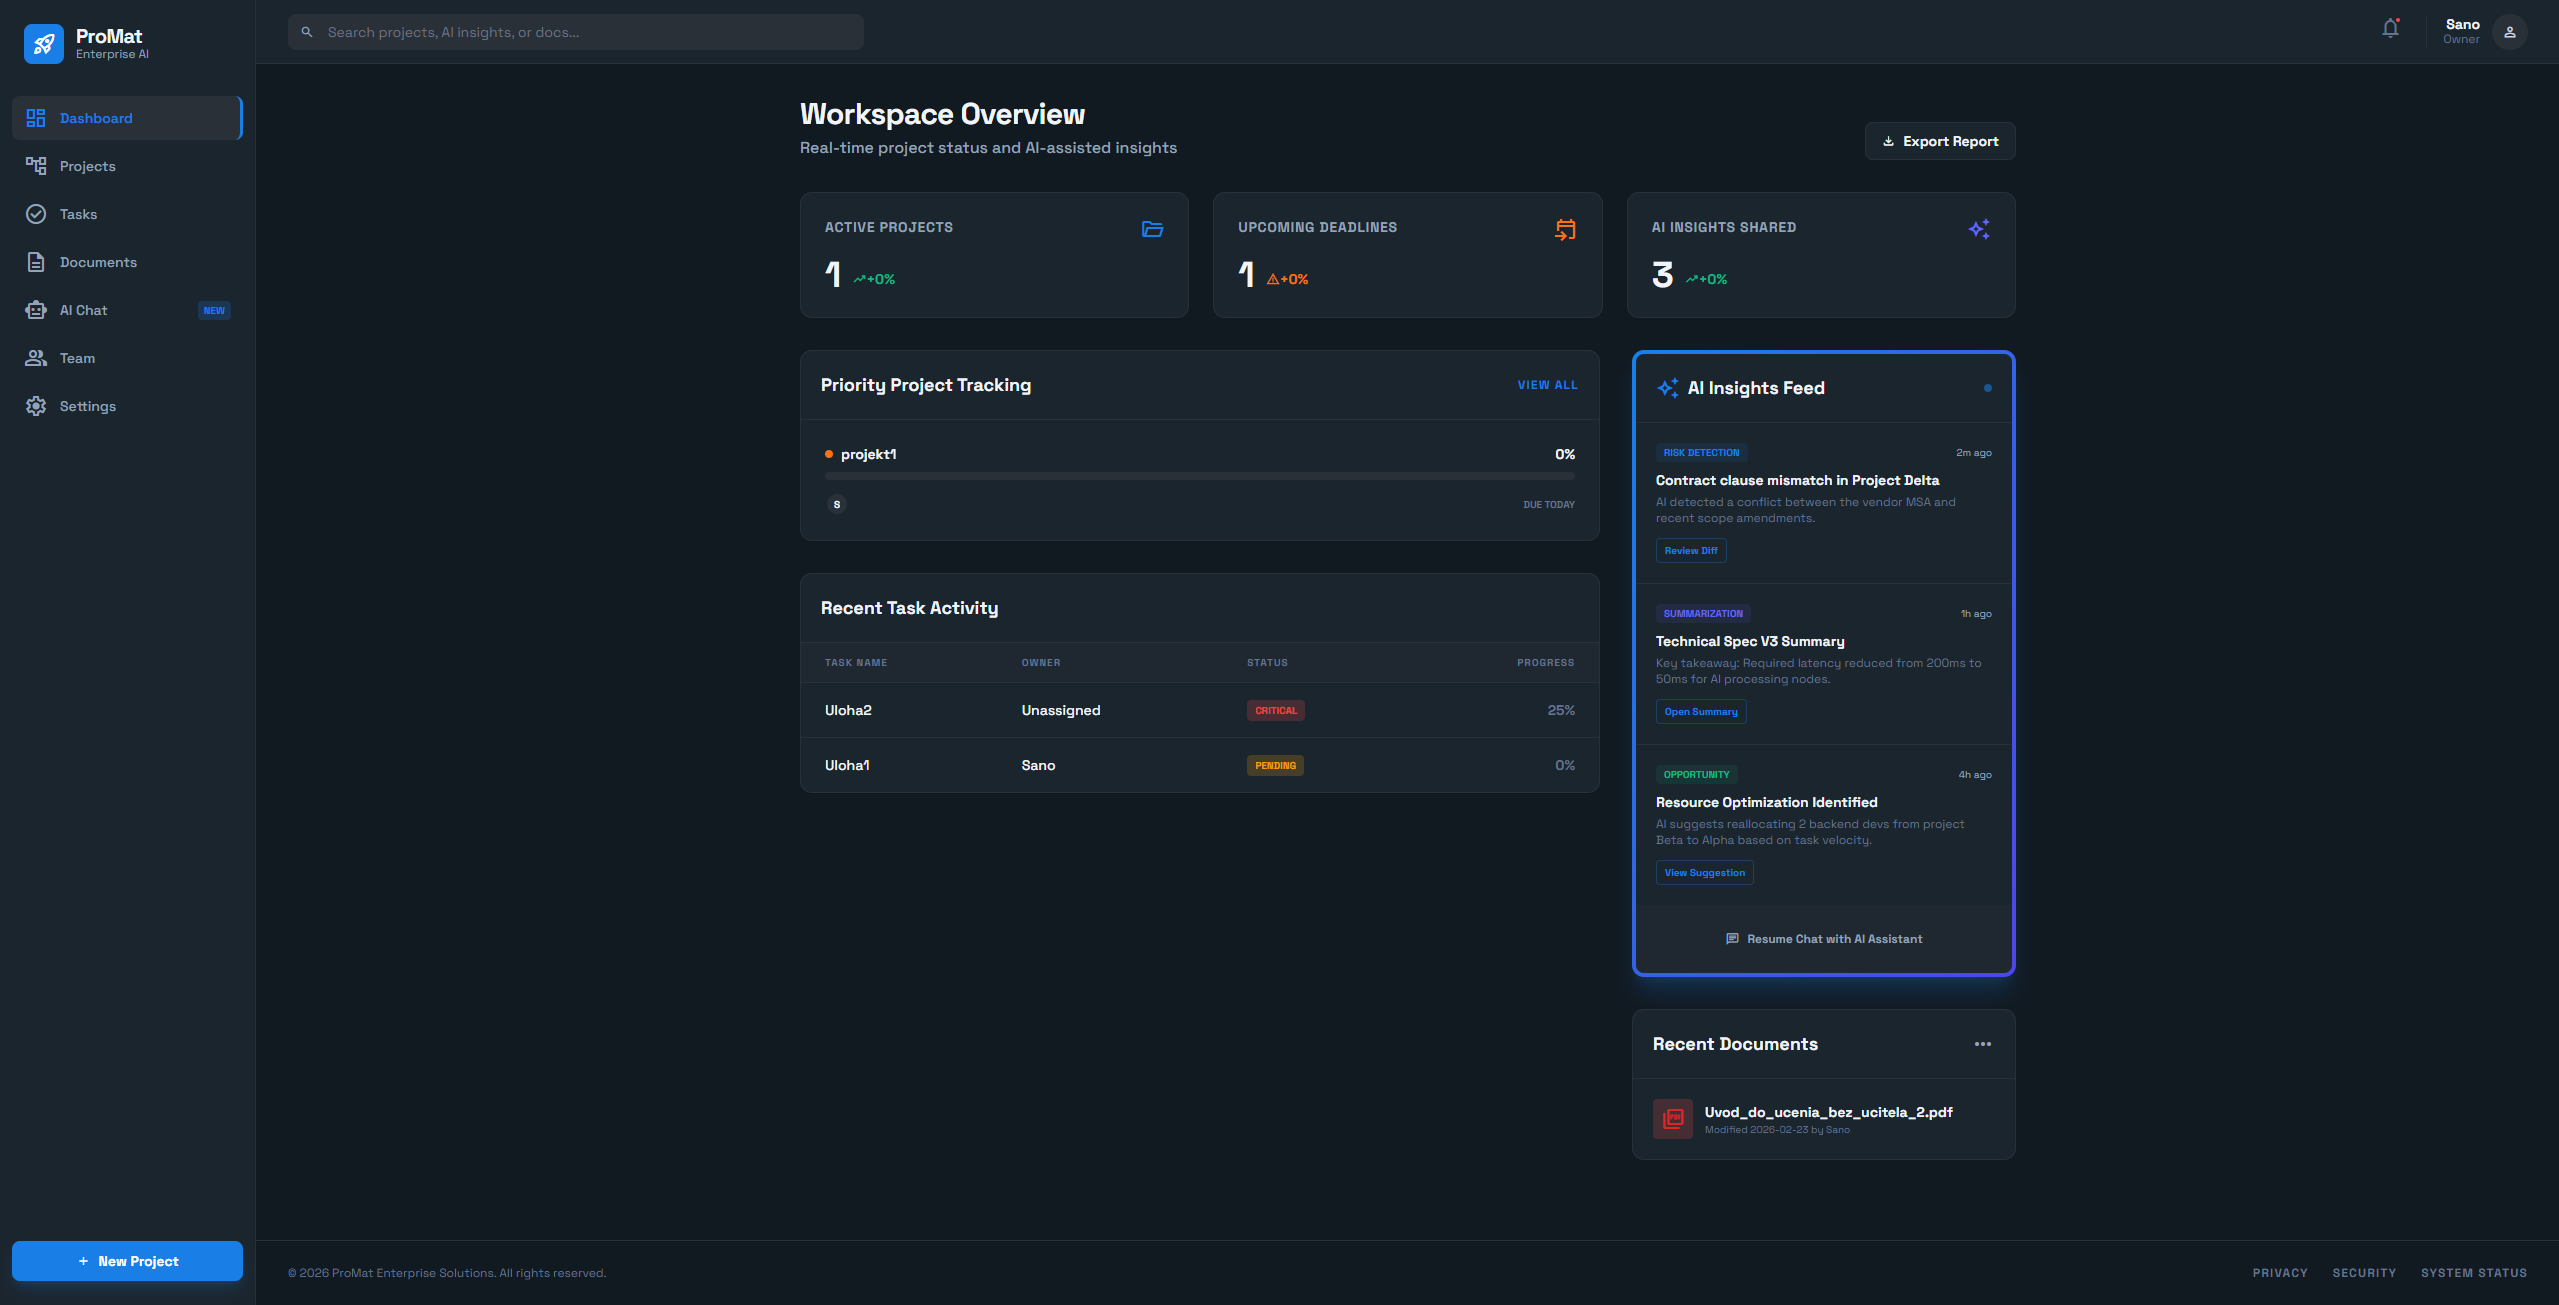
\includegraphics[width=0.95\textwidth]{dashboard.png}
    \caption{Dashboard aplikácie ProMAT}
    \label{fig:dashboard}
\end{figure}


\subsubsection{Interaktivita na klientovi}
Klientske skripty zabezpečujú najmä:
\begin{itemize}
    \item ovládanie bočného menu a modálnych okien,
    \item drag-and-drop operácie v kanban tabuli,
    \item dynamické správanie chat okna a asynchrónne odosielanie správ,
    \item pomocné interakcie (prepínanie filtrov, vizuálne potvrdenia akcií).
\end{itemize}

Použitím \textit{vanilla} JavaScriptu sme dosiahli nižšiu komplexitu závislostí a dobrú čitateľnosť kódu pre školský projekt, kde je dôležité, aby bola implementácia zrozumiteľná a ľahko obhájiteľná.

\subsection{Zhrnutie implementačnej časti}
Implementácia systému ProMAT prepája projektový manažment, správu dokumentov a AI funkcie do jedného celku. Architektúra je modulárna, dátový model pokrýva reálne tímové scenáre a používateľské rozhranie podporuje každodenné operácie bez zbytočnej zložitosti.

Rozšírenie o sprinty, reporty, notifikácie, integrácie a automatizačné pravidlá ukazuje, že aplikácia presahuje rámec jednoduchého CRUD systému a predstavuje plnohodnotnú platformu pre riadenie práce s dôrazom na praktické využitie v menších a stredných tímoch.

\subsection{Praktické prínosy riešenia pre tímovú prácu}
Pri implementácii sme sa nesústredili iba na technickú správnosť, ale aj na to, aby bol systém použiteľný v bežnej každodennej prevádzke menšieho tímu. Z praktického hľadiska sa ako najdôležitejší ukázal efekt centralizácie: projektové úlohy, dokumenty, komunikácia a plánovanie sú dostupné v jednom prostredí, bez potreby neustále prepínať medzi viacerými nástrojmi.

Významným prínosom je aj prepojenie medzi operatívnou prácou a znalosťami uloženými v dokumentoch. Pri riešení konkrétnej úlohy nemusí člen tímu manuálne prechádzať rozsiahle prílohy, ale môže sa opýtať AI vrstvy na konkrétny problém a okamžite získať odpoveď naviazanú na relevantný kontext. Takýto spôsob práce skracuje čas potrebný na orientáciu v podkladoch a zároveň znižuje riziko, že tím bude rozhodovať na základe neúplných informácií.

Za prakticky dôležité považujeme aj to, že architektúra systému umožňuje postupné rozširovanie podľa potrieb organizácie. Ak tím rastie alebo mení interné procesy, aplikáciu vieme rozširovať modulárne, napríklad o nové dashboard metriky, integračné body alebo automatizačné pravidlá, bez zásadného zásahu do existujúcich častí. Tento prístup zabezpečuje, že riešenie ostáva dlhodobo udržateľné a použiteľné aj po skončení školského projektu.

\newpage

% --- LITERATÚRA (ISO 690) ---
\renewcommand\refname{ZOZNAM BIBLIOGRAFICKÝCH ODKAZOV}
\begin{thebibliography}{99}

\bibitem{flask}
GRINBERG, Miguel. \textit{Flask Web Development: Developing Web Applications with Python}. 2nd ed. O'Reilly Media, 2018. ISBN 978-1491991732.

\bibitem{python}
Python Software Foundation. \textit{Python 3.12 Documentation} [online]. 2024. [cit. 2026-01-19]. Dostupné na: https://docs.python.org/3/

\bibitem{rag}
LEWIS, Patrick et al. \textit{Retrieval-Augmented Generation for Knowledge-Intensive NLP Tasks}. In: arXiv preprint arXiv:2005.11401, 2020.

\bibitem{sqlite}
OWENS, Mike. \textit{The Definitive Guide to SQLite}. Apress, 2006. ISBN 978-1590596739.

\bibitem{ollama}
Ollama. \textit{Ollama Documentation} [online]. 2024. [cit. 2026-01-19]. Dostupné na: https://ollama.ai/docs

\bibitem{agile}
BECK, Kent et al. \textit{Manifesto for Agile Software Development} [online]. 2001. [cit. 2026-01-19]. Dostupné na: https://agilemanifesto.org/

\end{thebibliography}

% --- PRÍLOHY ---
\newpage
\section*{PRÍLOHY}
\addcontentsline{toc}{section}{Prílohy}


\subsection*{Príloha A: Požiadavky (requirements.txt)}
\begin{verbatim}
Flask==3.0.0
Werkzeug==3.0.1
PyPDF2==3.0.1
python-docx==1.1.0
requests==2.31.0
numpy==1.26.0
langchain==0.1.0
\end{verbatim}


\label{LastPage}
\end{document}